% !TeX root=main.tex
\chapter{بررسی تاریخچه‌، مفاهیم اولیه و الگوریتم‌های پیش‌بینی برهم‌کنش دارو-دارو}



\section{پیشینه تحقیق}
\label{intro}
هنگامی که دو یا چند دارو باهم مصرف می‌شوند، اثرات دارویی یا رفتارهای آن‌ها به‌طور غیرمنتظره‌ای تحت تاثیر یکدیگر قرار می‌گیرند
\cite{Wienkers2005}. 
این نوع تاثیرگذاری به‌عنوان برهم‌کنش دارو-دارو نامیده می‌شود که می‌تواند تاثیر دارویی را کاهش دهد، مسمویت غیرمنتظره را افزایش دهد یا بین داروهای تجویز شده عوارض‌جانبی ایجاد کند. با افزایش داروهای تایید شده، تعداد برهم‌کنش‌ دارو-داروهای ناشناخته به سرعت در حال افزایش است، به‌طوری‌که در بین داروهای کوچک مولکول تایید شده در 
\lr{Drug‌Bank}،
به‌طور متوسط از هر یکصد جفت دارو تقریبا حدود پانزده‌تای آن‌ها دارای برهم‌کنش دارو-دارو هستند
\cite{Law2014}. 
برهم‌کنش دارو-داروهای ناشناخته باعث می‌شود بیمارانی که با چندین دارو تحت درمان هستند، در وضعیت ناایمن قرار گیرند
\cite{Leape1995, Businaro2013,Karbownik2017,Mulroy2017}. 
همچنین درک برهم‌کنش دارو-دارو اولین قدم برای ترکیب داروهاست که به یکی از راهکارهای امیدوارکننده برای درمان بیماری‌های پیچیده تبدیل می‌شود
\cite{Zhao2011}. 
بنابراین، غربالگری و تجزیه‌ و‌ تحلیل برهم‌کنش دارو-داروها قبل از تجویز بالینی داروها، یک نیاز فوری است. با‌این‌حال، رویکردهای سنتی برای شناسایی برهم‌کنش دارو-دارو (به‌عنوان مثال، در آزمایش 
\lr{Cytochrome P450}\cite{Veith2009} 
یا برهم‌کنش مربوط به انتقال‌دهنده‌ی دارو
\cite{Huang2007}) 
با چالش‌هایی روبه‌رو است. از آن جمله می‌توان هزینه‌های بالا، مدت زمانی طولانی، ملاحظات رفاه حیوانات
\cite{Zhang2015}، 
تعداد بسیار محدود شرکت‌کنندگان در آزمایش و تعداد زیاد ترکیبات دارویی تحت غربالگری آزمایش‌های بالینی را نام برد. تاکنون فقط تعداد کمی از برهم‌کنش دارو-داروها در طول تولید دارو شناسایی شده‌اند (معمولا در مرحله‌ی آزمایش بالینی). برخی از آن‌ها پس از تایید داروها گزارش شده‌اند و بسیاری از آن‌ها در نظارت بعد از عرضه پیدا شده‌اند.

رویکردهای محاسباتی جایگزین امیدوارکننده‌ای برای کشف برهم‌کنش دارو-داروهای بالقوه
\LTRfootnote{Potential}
در مقیاس گسترده هستند که بیش‌تر از گذشته، مورد استقبال دانشگاه و صنعت قرار گرفته‌اند
\cite{Wiśniowska2016, Zhou2016}.
رویکردهای محاسباتی مبتنی بر داده‌کاوی برای تشخیص برهم‌کنش دارو-دارو از منابع مختلف
\cite{Zhang2015}
از‌جمله: متون علمی
\cite{Bui2014, Zhang2016}،
سوابق پزشکی الکترونیکی
\cite{Duke2012}
و سیستم گزارش حوادث نامطلوب
\LTRfootnote{Event Reporting System}\lr{FDA}
استفاده می‌کنند. این رویکردها به شواهد بالینی پس از عرضه به بازار متکی هستند، بنابراین نمی‌توانند هشدارهایی از برهم‌کنش دارو-داروهای بالقوه را قبل از تجویز بالینی دارو ارائه دهند. در مقابل رویکردهای مبتنی بر یادگیری ماشین (رویکرد مبتنی بر شباهت نیو
\LTRfootnote{Naïve Similarity-Based Approach}\cite{Vilar2014}،
مبتنی بر گراف توصیه‌گر
\LTRfootnote{Network Recommendation-Based}\cite{Zhang2015}،
مبتنی بر طبقه‌بندی
\LTRfootnote{Classification-Based}\cite{Cheng2014})
قادر به ارائه‌ی چنین هشدارهایی با استفاده از ویژگی‌ها و شباهت‌های دارویی، قبل و بعد از ارائه به بازار هستند
\cite{Li2016}.

در این شیوه‌ها از ویژگی‌های مختلف دارو برای پیش‌بینی برهم‌کنش دارو-دارو استفاده می کنند، که عبارت‌اند از: ساختار شیمیایی
\cite{Vilar2014}،
هدف
\cite{luo2014}،
کدهای دسته‌بندی سلسله مراتبی
\LTRfootnote{Hierarchical Classification Codes}\cite{Cheng2014}
و تاثیرات جانبی
\cite{Zhang2015, Shi2017}.

بسیاری از رویکردهای مبتنی بر یادگیری ماشین برای پیش‌بینی دوکلاسه معمولی طراحی شده‌اند که تنها احتمال برهم‌کنش دارو-داروی یک جفت دارو را نشان می‌دهند، اما دو داروی برهم‌کنش پذیرفته‌شده ممکن است رفتارها یا اثرات دارویی خود را در بدن افزایش یا کاهش دهند.
به‌عنوان مثال:

۱) غلظت سرم
\lr{Flunisolide}
(با شناسه‌ی
\lr{DrugBank}،
\lr{DB00180})
وقتی با
\lr{Mitotane}
(با شناسه‌ی
\lr{DrugBank}،
\lr{DB00648})
به‌صورت هم‌زمان مصرف شود، کاهش می‌یابد.

۲) درحالی‌که غلظت همین سرم وقتی با 
\lr{Roxithromycin}
(با شناسه‌ی
\lr{DrugBank}،
\lr{DB00778})
هم‌زمان مصرف شود، افزایش می‌یابد.

مورد اول را برهم‌کنش دارو-داروی کاهنده
\LTRfootnote{Degressive}
و دومین مورد را برهم‌کنش دارو-داروی افزاینده
\LTRfootnote{Enhancive}
می‌نامیم و هر دو مورد را به‌عنوان برهم‌کنش دارو-دارو که شامل تاثیرات دارویی موثر هستند در نظر می‌گیریم. دانستن دقیق این نکته که برهم‌کنش باعث افزایش یا کاهش تاثیر دارو می‌شود، به‌ویژه در هنگام مراقبت از بیمار، تعیین مقدار مصرف دارو، طراحی دارو یا یافتن مقاومت دارو در برابر درمان، بسیار مهم است
\cite{Koch1981}.
بسیاری از رویکردهای موجود هنوز از این خاصیت ساختاری استفاده نکرده‌اند و فقط برای برهم‌کنش دارو-داروهای دوکلاسه معمولی توسعه یافته‌اند. درحالی‌که شناخت نوع برهم‌کنش دارو-دارو، یکی از مهم‌ترین اقدامات برای درمان بیماری‌های پیچیده است
\cite{Cokol2017}
و می‌تواند راهنمای پزشکان در تهیه نسخه‌های مطمئن‌تر باشد. در ادامه سه روش برای پرداختن به موارد ذکر شده توضیح داده می‌شود. این سه روش از پیش‌بینی‌های سه‌کلاسه جامع به‌جای پیش‌بینی دوکلاسه معمولی استفاده کردند و به بررسی ساختاری داروها در شبکه برهم‌کنش داروها پرداختند.


در بخش بعدی روش‌های آماده‌‌سازی داده و رویکردهای انتخاب مدل، به‌کار رفته در مقالات پیشین، فرمول‌بندی و توضیح داده می‌شوند. مطالعه‌ی این بخش کمک شایانی به‌درک فرآیند به‌کار رفته در روش پیشنهادی می‌کند.


\section{آماده‌سازی داده}
\label{dataPreparing}
 
در این بخش به بحث در مورد روش‌های متداول محاسبه‌ی شباهت‌های دارویی و ترکیب شباهت‌های شبکه‌ای می‌پردازیم.

\subsection{محاسبه‌ی شباهت‌های دارویی
\label{simCal}}

سه روش متداول محاسبه‌ی شباهت که در مقالات یادگیری ماشین مانند مقالات
\cite{FWang2008,WZhang2016, WZhang2017}
 استفاده می‌شوند، عبارت‌اند از:
\textbf{شباهت جاکارد}\LTRfootnote{Jacard Similarity}،
\textbf{شباهت کوسینوس}\LTRfootnote{Cosine Similarity}
و
\textbf{شباهت گوسین}\LTRfootnote{Gaussian Similarity}. 
این روش‌ها مقدار شباهت بین دو نمونه داده را منعکس می‌کنند و به‌طور گسترده در بیوانفورماتیک مورد استفاده قرار گرفته‌‌اند
\cite{WZhang2017, WZhang20171, WZhang20172, WZhang2018_1, WZhang2018_2}.
اگر بردارهای ویژگی دارو
$d_i$
و
$d_j$
را با
$x_i$
و
$x_j$
نمایش دهیم، سه روش شباهت به شرح زیر تعریف می‌شوند:


\begin{itemize}
\item شباهت جاکارد بین
$x_i$ 
و
$x_j$ 
\begin{equation}
\begin{aligned}
S_{Jar}(x_i,x_j) =\dfrac{N_{11}}{N_{10} + N_{01} + N_{11}}
\end{aligned}
\end{equation}
که:

$N_{11}$ 
تعداد کل عناصری است که
$x_i$
و
$x_j$
هر دو مقدار 1 گرفته اند. 
 
$N_{10}$ 
تعداد کل عناصری است که
$x_i$ 
مقدار 1 و
$x_j$
مقدار 0 گرفته‌اند. 
  
$N_{01}$ 
تعداد کل عناصری است که
$x_i$
مقدار 0 و 
$x_j$ 
مقدار 1 گرفته‌اند. 

\item شباهت کوسینوس بین
$x_i$
و 
$x_j$
\begin{equation}
\begin{aligned}
S_{Cos}(x_i,x_j) =\dfrac{x_i . x_j}{||x_i||_2 ||x_j||_2}
\end{aligned}
\end{equation}
که
$||~||_2$
نرم اقلیدسی است و
${x_i . x_j}$
ضرب داخلی دو بردار را نمایش می‌دهد.


\item شباهت گوسین بین
$x_i$
و 
$x_j$
\begin{equation}
\begin{aligned}
S_{Gau}(x_i,x_j) = exp(-\sigma ||x_i - x_j||_2^2)
\end{aligned}
\end{equation}
که
$\sigma  (>0)$
پارامتر پهنای باند است و به‌صورت
$\sigma  =\dfrac{1}{\sum _{i=1}^m \dfrac{|x_i|}{m}}$
تنظیم می‌شود.
\end{itemize}

سایر روش‌های محاسبه شباهت بین دو دارو در شکل
\ref{fs7}
نمایش داده شده ‌است.
\begin{figure}[!h]
	\centering
	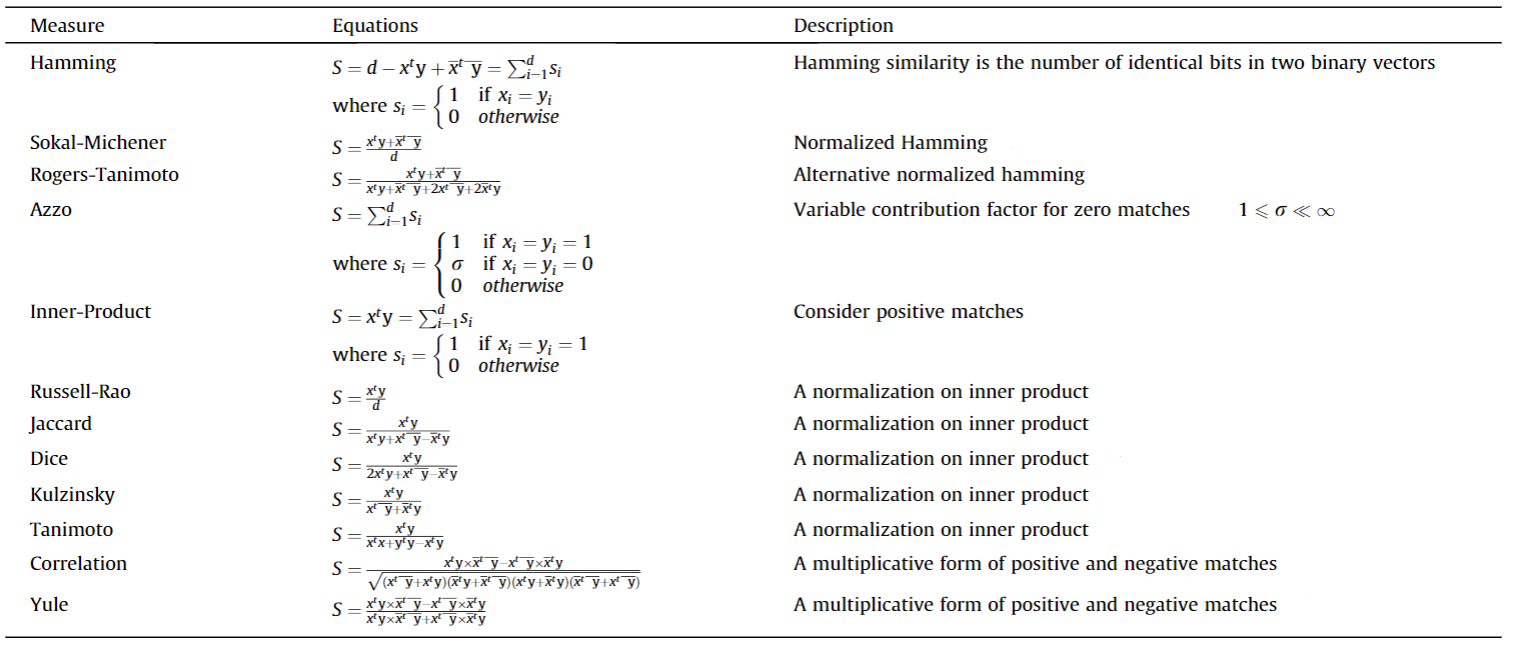
\includegraphics[scale=0.63]{section1/sims.png}
	\caption{انواع شباهت بین بردارهای دودویی}
	\label{fs7}
\end{figure}

\subsection{ترکیب شباهت‌های شبکه‌ای
\label{SNF}}

ترکیب شباهت‌های شبکه‌ای
\LTRfootnote{Similarity Network Fusion}\cite{Wang2014}\lr{(SNF)}
یک روش محاسباتی جدید برای ترکیب داده‌ها است. این روش انواع مختلفی از ویژگی‌ها (مانند ساختار شیمیایی، عوارض‌جانبی، آنزیم، منتقل‌کننده و غیره) را با مجموعه‌ی معینی از نمونه‌ها (به‌عنوان مثال داروها) ترکیب می‌کند. در این روش ابتدا برای هر یک از انواع داده‌ها یک شباهت نمونه ایجاد می‌شود و سپس با استفاده از یک روش جدید ترکیب شبکه،‌ شبکه‌ها یکپارچه می‌شوند. کار در فضای شبکه به
\lr{SNF}
اجازه می‌دهد تا از برخورد با مقیاس‌های مختلف، اریبی
\LTRfootnote{Bias}
 و نویز در انواع مختلف داده جلوگیری کند. روش ترکیب غیرخطی داده‌ها به
\lr{SNF} 
اجازه می‌دهد تا هم از اطلاعات رایج و هم از اطلاعات مکمل در انواع مختلف داده استفاده برد. شکل
\ref{fs8}
مثالی از مراحل
\lr{SNF} 
است.
 

\begin{figure}[!h]
	%\centering
	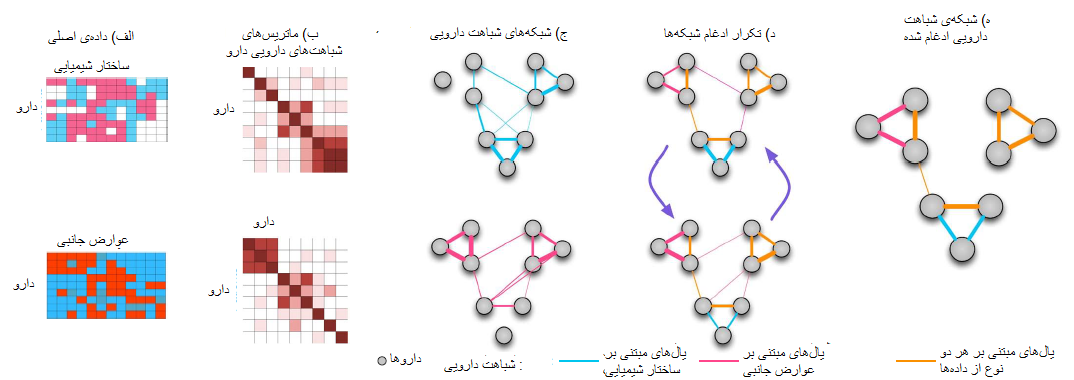
\includegraphics[scale=0.57]{section2/SNF.png}
	\caption{انواع شباهت بین بردارهای دودویی
    \cite{Wang2014}}
الف) نمایش نمونه‌ای از ویژگی ساختار شیمیای و ویژگی عوارض‌جانبی خارج از برچسب برای همان داروها. ب) ماتریس تشابه دارو-دارو برای هر نوع ویژگی. ج) شبکه‌های شباهت دارو-دارو، معادل داده‌های دارو-دارو.داروها توسط گره‌ها نمایان می‌شوند و شباهت‌های جفتی داروها توسط یال‌ها نشان داده ‌می‌شود. د) تلفیق شبکه توسط
\lr{SNF}
به‌طور مکرر، هر یک از شبکه‌ها را با اطلاعاتی از شبکه‌های دیگر به روز می‌کند و آن‌ها را در هر مرحله شبیه‌تر می‌کند. ه) ترکیب شبکه به‌صورت تکراری منجر به همگرایی می‌شود. رنگ یال نشان می‌دهد که کدام نوع داده به شباهت داده‌شده کمک کرده ‌است.
	\label{fs8}
\end{figure}

\section*{انتخاب مدل}

در این بخش توضیح مختصری از تاریخچه‌ی سامانه‌های توصیه‌گر و یادگیری عمیق داده می‌شود و سپس به بررسی تقسیم‌بندی آنها می‌پردازیم.

\section{سامانه‌های توصیه‌گر}

به کمک کامپیوتر‌ جوامع امروزی دستخوش تغییرات سریعی شده‌اند. بخش قابل توجهی از زندگی اجتماعی را کامپیوتر و اینترنت در برگرفته ‌است. یکی از موضوعات جدید مورد بحث حال حاضر دنیای کامپیوتر، سامانه‌های توصیه‌گر می‌باشد.

سامانه‌های توصیه‌گر
\LTRfootnote{Recommender Systems}
با اولین ظهورشان در زمینه فیلترینگ همکارانه
\LTRfootnote{Collaborative Filtering}،
حوزه تحقیقاتی مهمی را در اواسط دهه ۱۹۹۰ فراهم نمودند. دردهه‌های اخیر دو بخش صنعت و دانشگاه دستاوردهای جدیدی در زمینه سامانه‌های توصیه‌گر توسعه داده‌اند، با این ‌وجود علاقه‌مندی به این بخش هنوز در سطح بالایی است. تحقیقات این حوزه غنی بوده و نیاز مبرم به برنامه‌های کاربردی وجود دارد. این برنامه‌های کاربردی به‌منظور کمک به کاربران که با حجم زیادی از اطلاعات مواجه هستند و به‌منظور شخصی‌سازی اطلاعات توسعه داده شدند. به‌عنوان مثال از چنین برنامه‌هایی، می توان به سامانه‌های توصیه‌گر کتاب، سی‌دی و دیگر محصولات سایت آمازون
\LTRfootnote{Amazon}
و پیشنهاد فیلم توسط شرکت موی‌لنز
\LTRfootnote{MovieLens}
اشاره کرد.

تقریبا در اواسط دهه نود، مطالعه بر روی سامانه‌های توصیه‌گر به‌عنوان یک شاخه مستقل در تحقیقات مطرح شد. علت این توجه خاص، ابراز تمایل محققین، به‌استفاده از سامانه‌های توصیه‌گر برای حل مسئله جستجو در حجم فراوان اطلاعات بود. ظرفیت کامپیوترها در فراهم آوردن توصیه‌ها تقریبا از همان اوایل تاریخچه کامپیوتر‌ها شناخته شد. گراندی
\LTRfootnote{Grundy}،
کتابدار کامپیوتری گامی اولیه به سمت سامانه‌های توصیه‌گر خودکار برداشت. این کتابدار یک توصیه‌گر نسبتا ساده و اولیه بود که کاربران را به قالب‌هایی براساس مصاحبه کوتاه با استفاده از اطلاعات مستقیم‌کدشده
\LTRfootnote{Hard-coded}
درباره‌ی سلایق کتاب قالب‌های مختلف گروه‌بندی می‌کرد تا توصیه‌ها را تولید کنند. این کار ورود اولیه به فضای سامانه‌های توصیه‌گر قلمداد می‌شود.

در اوایل دهه نود میلادی، تکنیک پالایش مشارکتی
\LTRfootnote{Collaborative Refinement}
 به‌عنوان راه‌حلی برای مدیریت فضای اطلاعات بسیار زیاد آنلاین به‌وجود آمد. تپستری
\LTRfootnote{Tapestry}
یک سامانه پالایش مشارکتی دستی بود. این سامانه به کاربر اجازه انجام پرس‌وجو برای آیتم‌های موجود در حوزه اطلاعاتی مانند ایمیل بر اساس عقاید و اقدامات دیگر کاربران را می‌داد. این‌کار مستلزم تلاش از طرف کاربران بود و به آنها اجازه کنترل واکنش‌های خوانندگان قبلی در قسمتی از مکاتبات را می‌داد تا میزان ارتباط با آنها را تعیین کند. خیلی زود بعد از سامانه‌های خودکار پالایش مشارکتی، مکان‌یابی خودکار عقاید مرتبط و تجمع آنها برای دادن توصیه مطرح شد. گروپ لنز
\LTRfootnote{Group Lens}
از این تکنیک برای تعیین مقاله‌های یوزنت
\LTRfootnote{Usenet}
که احتمال دارد مورد علاقه کاربر خاصی باشد استفاده کرد. کاربران تنها به نمره‌دهی یا دیگر اقدامات قابل مشاهده می‌پرداختند. سامانه این فعالیت‌ها را با نمره‌ها یا اقدامات دیگر کاربران ترکیب می‌کرد تا نتایج شخصی‌شده تولید کند. با این سامانه‌ها، کابران برای دریافت پیشنهادات، قادرند بدون آنکه بدانند کاربران یا آیتم‌های دیگر سامانه چه‌چیزهایی هستند، اطلاعات مستقیمی از عقاید دیگر کاربران بدست آورند.

طی این دوره، سامانه‌های توصیه‌گر و پالایش مشارکتی تبدیل به موضوع مورد علاقه محققین حوزه‌های تعاملات انسان-رایانه، یادگیری ماشین و بازیابی اطلاعات شدند. این علاقه منجر به ایجاد سامانه توصیه‌گر در زمینه‌های مختلف شد. که از آن جمله می‌توان به
\lr{Ringo}
برای موسیقی، توصیه‌گر ویدیو 
\lr{BellCore}
برای فیلم‌ها و 
\lr{Jester}
برای لطیفه‌ها اشاره کرد. خارج از دنیای رایانه و درحوزه بازاریابی از توصیه‌گر‌ها، به‌دلیل توانایی آنها در افزایش فروش و بهبود تجربه مشتریان، استفاده کرده‌اند.

در اواخر دهه نود میلادی، پیاده‌سازی‌های تجاری فناوری توصیه‌گرها شروع به‌ظهور کردند. شاید معروف‌ترین کاربرد فناوری سامانه‌های توصیه‌گر وب‌سایت
\lr{Amazon.com}
باشد. براساس تاریخچه خرید، تاریخچه بازدید و موردی که کاربر درحال مشاهده است، وب‌سایت به کاربر مواردی را برای خرید توصیه می‌کند. از زمان به‌کارگیری فناوری توصیه‌گر توسط آمازون، در بسیاری از سیستم‌های تجارت الکترونیک و آنلاین، سامانه‌های توصیه‌گر (که اغلب بر اساس پالایش مشارکتی هستند)، ایجاد شده است. انگیزه مهم انجام این‌کار افزایش حجم فروش است زیرا ممکن است اگر کالا‌یی به مشتریان پیشنهاد شود آن را بخرند و درغیراینصورت ممکن است هرگز متوجه آن کالا نشده و آنرا نخرند. شرکت‌های بسیاری مانند 
\lr{NetPerceptions}
و 
\lr{Strands}
به‌دلیل فراهم‌کردن فناوری و خدمات توصیه به خرده‌فروشان آنلاین بوجود آمده‌اند.

زمانی‌که
\lr{Netflix}
جایزه 
\lr{Netflix Prize}
را در سال ۲۰۰۶ به منظور بهبود بخشیدن وضعیت توصیه‌های فیلمش برقرار کرد، تحقیق بر روی الگوریتم‌های سامانه‌های توصیه‌گر توجه بسیاری را به خودش جلب کرد. هدف این رقابت ساختن الگوریتم توصیه‌گری بود که بتواند الگوریتم
\lr{CineMatch}
که متعلق به خود
\lr{Netflix}
بود را با ۱۰٪ بهبود در آزمایشات آفلاین شکست دهد. این امر موجب ایجاد اقدامات گسترده‌ای در محیط دانشگاهی و سایر علاقمندان شد. جایزه یک میلیون دلاری ارزشی که فروشندگان برای دقت توصیه‌ها قائل هستند را نشان می‌دهد
\cite{HCI-009}.
به‌طور کلی دلیل استفاده از سامانه‌های توصیه‌گر و فیلترینگ اطلاعات، تبدیل اطلاعات موجود در مورد کاربران و اولویت‌های آن‌ها جهت پیش‌بینی علاقه آنها در آینده می‌باشد. در واقع در این سامانه از بین موارد مختلف بر اساس اینکه چه موردی برای کاربر جذاب است، مجموعه‌ی بزرگی از موارد مورد علاقه کاربران جمع‌آوری می‌شود. وب‌سایت‌های زیادی مانند
\lr{Amazon}، \lr{CDnow}، \lr{Ebay}
و غیره شروع به استفاده از سامانه‌های توصیه‌گر برای اهداف فروش الکترونیکی کردند. این وب‌سایت‌ها با توجه به اطلاعات و علایق مشتری به مشتری محصول مناسب سلیقه او را پیشنهاد می‌دهند که سبب افزایش رابطه میان وب‌سایت‌ها و مشتریان می‌شود. این باور وجود دارد که با ارائه توصیه‌های با کیفیت به مشتری و جلب رضایت او، وفاداری مشتری بهبود می‌یابد.

پیشرفت اینترنت باعث شده است اطلاعات آنلاین زیادی قابل دسترسی باشد. سامانه‌های توصیه‌گر می‌توانند مشکل انباشت اطلاعات را حل کنند. هدف این سامانه‌ها شناسایی سلیقه‌های کاربران و فیلترکردن داده‌های نامناسب از نظر آنهاست. نتیجه استفاده از سامانه‌های توصیه‌گر صرفه‌جویی زمانی جستجوهای کاربران است.
در شکل
\ref{recom1}
شمای کلی فرایند توصیه در سامانه‌های توصیه‌گر را مشاهده می‌کنید.


\begin{figure}
	\centering
	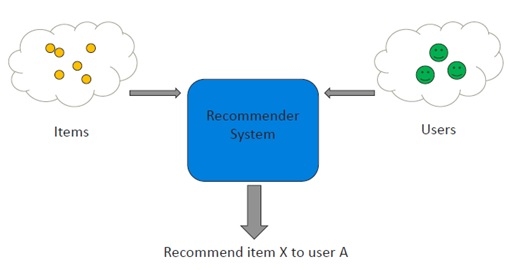
\includegraphics[scale=0.8]{section2/Recom1.jpg}
	\caption{شمای کلی فرایند توصیه در سامانه‌های توصیه‌گر}
	\label{recom1}
\end{figure}

\subsection*{تقسیم‌بندی سامانه‌های توصیه‌گر}

در کتاب‌های مختلف تقسیم بندی‌های مختلفی برای سامانه‌های توصیه‌گر وجود دارد. معمول‌ترین تقسیم‌بندی سامانه‌های توصیه‌گر را می‌توانید در شکل
\ref{Recom}
 مشاهده کنید.
 
\begin{figure}
\centering
\begin{tikzpicture}
        [edge from parent fork left, grow=left,
        every node/.style={fill=red!10,rounded corners},
        edge from parent/.style={gray,thick,draw}]
        \tikzstyle{block} = [ text width=4cm,text centered, minimum height=1em, fill=red!15]
        \tikzstyle{level 1}=[sibling distance=18mm,level distance=55mm] 
		\tikzstyle{level 2}=[sibling distance=15mm,level distance=55mm] 
        \node [block]{\lr{Recommendr Systems}}
	child{node[block] {\lr{Collabortive Filtrring}}
    	child{node[block]{\lr{User-Based}\rl{}}}
        child{node[block]{\lr{Item-Based}\rl{}}}
    	child{node[block]{\lr{Matrix Factorization}\rl{}}}
	}
	child{[sibling distance=5mm]node[block] {\lr{Content-Based }}
	}
	child{node[block] {\lr{Knowledge-Based}}
    	child{node[block]{\lr{Constrain-Based}\rl{}}}
    	child{node[block]{\lr{Case-Based}\rl{}}}
	}
	child{node[block] {\lr{Hybrid Approaches}}
	};

\end{tikzpicture}
	\caption{
تقسیم‌بندی سامانه‌های توصیه‌گر
\cite{HCI-009}
}
\label{Recom}
\end{figure}

\subsection{فیلترینگ همکارانه}
در روش فیلترینگ همکارانه
\LTRfootnote{Collabortive Filtrring}
پیشنهادات براساس شباهت‌های رفتاری و الگوهای عملکردی کاربرانی که شباهت‌های رفتاری و الگوهای مشابهی با کاربر فعلی در گذشته داشته‌اند، ارائه می‌شود. شاید تعریف آن کمی پیچیده باشد، به‌طور ساده روش فیلترینگ همکارانه بر این فرض استوار است که کاربرانی با نظرهای مشابه درباره یک مورد (منظور فیلم، عکس، موزیک یا هر چیز دیگری است که توصیه می‌شود) دارند، درباره موارد دیگر هم نظرات مشابه دارند. نمای کلی عمکرد این روش را در شکل
\ref{recom3}
مشاهده کنید. فیلترینگ همکارانه شامل سه بخش است که به بررسی آن‌ها می‌پردازیم:
\begin{figure}
	\centering
	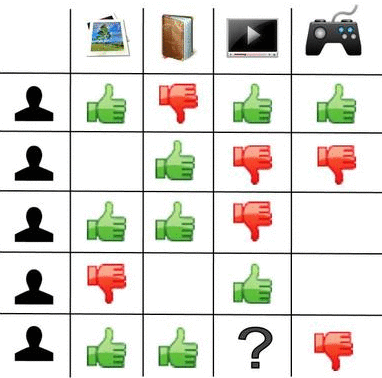
\includegraphics[scale=0.6]{section2/recom3.png}
	\caption{نمای کلی از روش‌های فیلترینگ همکارانه}
	\label{recom3}
\end{figure} 

\begin{itemize}
\item \textbf{مبتنی بر کاربر \LTRfootnote{User-Based}:}
در این روش افراد هم سلیقه با توجه به امتیازاتی که به موارد داده‌اند دسته‌بندی می‌شوند. از آنجا که کاربرانی با سلیقه شبیه به فرد مورد نظر بود و از  موارد یکسان خوششان آمده بود، پس آن مورد را به فرد مورد نظر نیز پیشنهاد می‌دهند.
\item \textbf{مبتنی بر آیتم \LTRfootnote{Item-Based}:}
در این روش وقتی یک کاربر یک مورد را می‌بیند، سامانه به‌صورت خودکار به دنبال آن می‌گردد که کاربرانی که قبلا این مورد را دیده‌اند بعد از آن چه موارد دیگری را دیده بودند. سپس سامانه آن موارد را به کاربر پیشنهاد می‌دهد. مثلا در سایت آمازون اگر یک گوشی بخرید بعد از آن، سامانه توصیه‌گر قاب گوشی و محافظ صفحه نمایشگر و چیزهایی مربوط به گوشی توصیه می‌کند.
\item \textbf{
تجزیه ماتریس
\LTRfootnote{Matrix Factorization}:\label{MatFactor}}
روش‌های مبتنی بر کاربر و مبتنی بر آیتم ساده هستند، اما معمولا روش‌های تجزیه ماتریس بیشتر تاثیرگذار هستند. زیرا این روش‌ها، ویژگی‌های پنهانی که در ارتباط میان کاربران و موارد وجود دارد را کشف می‌کنند. از این روش برای پیش‌بینی امتیازها در فیلترینگ همکارانه استفاده می‌کنند.
روش تجزیه ماتریس یک ماتریس ورودی را می‌گیرد و تلاش می‌کند دو ماتریس دیگر را به‌گونه‌ای بیابد که درصورت ضرب شدن در هم، ماتریس ورودی را تقریب بزنند. الگوریتم تجزیه ماتریس با مثال معروف توصیه‌ی کالاهای دیده نشده به کاربر معرفی می‌شود. در این حالت ماتریسی به‌نام
\lr{Y}
حاوی بازخوردهای کاربران برروی کالاها می‌باشد که شامل
\lr{m}
کاربر و
\lr{n}
کالا می‌باشد. مطابق شکل
\ref{Matrixfactorization}،
برای پیش‌بینی بازخورد کاربران روی کالاهای دیده ‌نشده ماتریس
$Y\epsilon R^{(m \times n)}$
به دو ماتریس
$A\epsilon R^{(m \times k)}$
و
$B\epsilon R^{(k \times n)}$
تقسیم می‌شود به‌طوری که
$ AB^T \approx Y$.
پارامتر قابل تنظیم
\lr{k}،
مربوط به تعداد ویژگی‌های نهفته
\lr{A} و \lr{B}
است كه
$k\ll m \times n$.

تجزیه ماتریس ویژگی‌های پنهان کاربران و کالاها را به شیوه‌ی بدون سرپرست مشخص می‌كند، كه برای فیلتركردن مشاركتی مفید است. به عنوان مثال، اگر بردارهای پنهان دو کاربر شبیه باشند، احتمال بالایی دارد که این کاربرها بازخوردهای یکسانی را به اشتراک بگذارند. به این ترتیب احتمال بازخورد مشابه روی کالاهای یکسان یا کالاهای مشابه بالاتر خواهد بود.

هدف يافتن بازخوردهای ناموجود در ماتریس
\lr{Y}
است كه تجزیه ماتریس می‌تواند به‌عنوان تکنیک تکمیل‌کننده‌ی ماتریسی مورد استفاده قرار گیرد. تصویری از تجزیه ماتریسی در شکل
\ref{Matrixfactorization}
نمایش داده شده‌است.

\begin{figure}[h!]
	\centering
	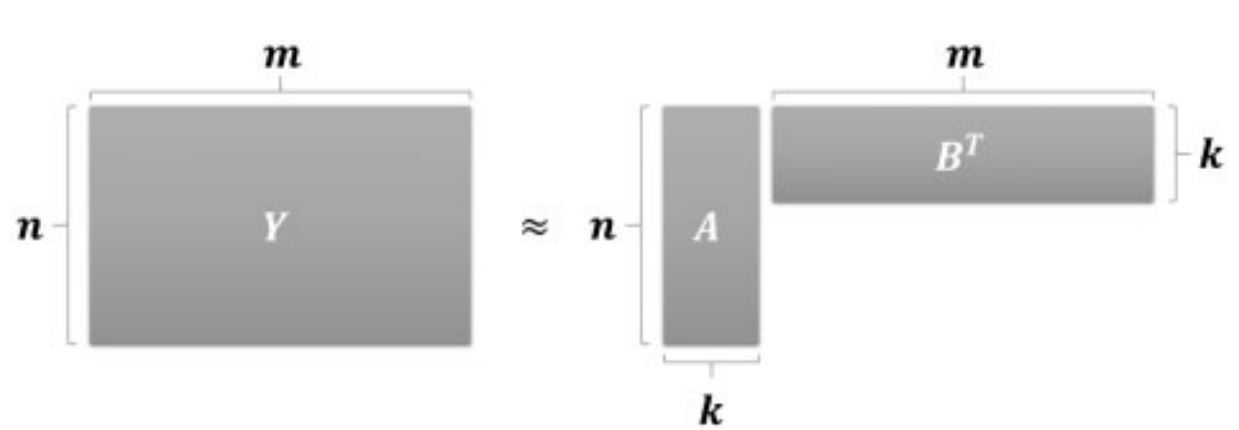
\includegraphics[scale=0.47]{section2/Matrixfactorization.jpg}
	\caption{
شرح مصور از تجزیه ماتریس}
\begin{flushright}
هدف این است که دو ماتریس ویژگی‌های پنهان
\lr{A} و \lr{B}
را به‌گونه‌ای بیابیم که ماتریس بازخورد
\lr{Y}
از ضرب این دو ماتریس بهتر بازسازی شود
\cite{Ezzat2018}.
\end{flushright}

	\label{Matrixfactorization}
\end{figure}


\end{itemize}
\par
\subsection{فیلترینگ مبتنی بر محتوا}

فیلترینگ مبتنی بر محتوا
\LTRfootnote{Content-Based}
از اطلاعات متنی و سابقه‌های کاربر برای تطابق موارد استفاده کرده و گزینه‌های مناسب را پیشنهاد می‌دهد. دانش اصلی‌ که در این تکنیک استفاده می‌شود شامل اطلاعات مواردی مثل ژانر، سال تولید و …  است که براساس این اطلاعات، مواردی که شبیه به هم هستند توصیه می‌شوند. در شکل 
\ref{recom4}
نحوه کلی عملکرد این روش را مشاهده می‌کنید. نمونه عمده این روش در وب‌سایت آمازون برای پیشنهاد کتاب‌ها بر اساس کلمات کلیدی کتاب‌های مشابه که سابقا توسط کاربر خریداری شده استفاده می‌شود.
\begin{figure}
	\centering
	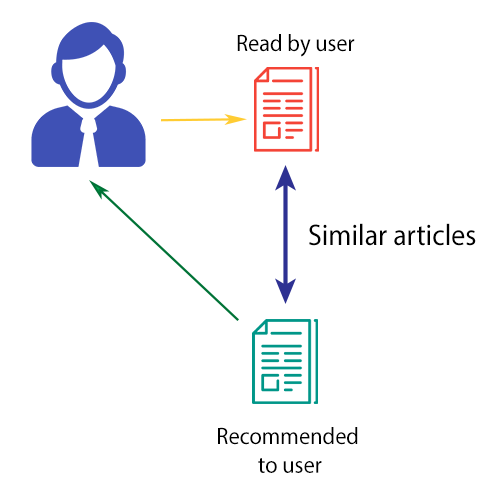
\includegraphics[scale=0.5]{section2/recom4.png}
	\caption{نمای کلی از روش‌های فیلترینگ مبتنی بر محتوا}
	\label{recom4}
\end{figure}
\par
\subsection{فیلترینگ مبتنی بر دانش}
دو روش توصیه‌گر قبلی محدودیت‌هایی دارند. محدودیت‌های استفاده از فیلترینگ همکارانه و فیلترینگ مبتنی بر محتوا را می‌توانید در قالب مثال بعدی ببینید. معمولا افراد به‌صورت مکرر ماشین، خانه و یا کامپیوتر نمی‌خرند. در این سناریوها یک سامانه فیلترینگ همکارانه خوب عمل نمی‌کند چون تعداد امتیازهای موجود بسیار کم است. علاوه‌بر‌این، محدوده زمانی نقش بسیار مهمی ایفا می‌کند. برای مثال، امتیازهایی که پنج سال قبل به یک کامپیوتر داده شده‌است به طور قطع برای توصیه مبتنی بر محتوا مناسب نیست.

روش فیلترینگ مبتنی بر دانش
\LTRfootnote{Knowledge-Based}
چالش‌های ذکرشده را حل می‌کند. سامانه‌های توصیه‌گر مبتنی بر دانش، نسل جدیدی از سامانه‌های توصیه‌گر هستند که مبتنی بر دانش موجود در رابطه با کاربران و موارد هستند. چنین سامانه‌هایی، پیشنهادات خود را بر پایه تفسیر و استنباط خود از سلایق و نیاز‌های کاربر ارائه می‌دهند و از دیدگاه تئوری نسبت به سایر روش‌های ذکر شده از دقت و کیفیت بیشتری برخوردار هستند. برای پیاده‌سازی چنین سامانه‌هایی نیاز به یک بستر و ساختار مبتنی بر دانش وجود دارد. در این گونه سامانه‌های توصیه‌گر موارد اولیه مورد استفاده برای تولید لیستی از پیشنهادها، دانش سامانه درمورد مشتری و کالا است. سامانه‌های مبتنی بر دانش از روش‌های مختلفی که برای تحلیل دانش قابل استفاده هستند بهره می‌برند. روش‌های رایج در الگوریتم‌های ژنتیک
\LTRfootnote{Genetic Algorithms}،
فازی
\LTRfootnote{Fuzzy}،
شبکه‌های عصبی
\LTRfootnote{Artificial Neural Networks} 
و … از جمله آنها است. همچنین، در این سامانه‌ها از درخت‌های تصمیم
\LTRfootnote{Design Tree}،
استدلال نمونه ‌محور
\LTRfootnote{Case-Based Reasonong}
و … نیز می‌توان استفاده کرد. روش مبتنی بر دانش خود به دو روش مبتنی بر محدودیت 
\LTRfootnote{Constrain-Based}
و مبتنی بر مورد 
\LTRfootnote{Case-Based}
تقسیم می‌شود. هر دو روش از لحاظ فرایند توصیه یکی هستند یعنی اول یک کاربر باید بطور دقیق درخواست خود را بگوید سپس سامانه تلاش ‌کند که یک راه‌حل تشخیص بدهد. سامانه حتی می‌تواند توضیح کوتاهی برای دلیل توصیه مورد بدهد. اما این دو روش از لحاظ تهیه دانش باهم تفاوت دارند. روش مبتنی بر مورد، آیتم‌های مشابه را با استفاده از میزان تشابه 
\LTRfootnote{Similarity Measure}
توصیه می‌کند اما روش مبتنی بر محدودیت، با توجه به قانون‌های توصیه‌ای که از قبل به طور صریح تعبیه شده فرایند توصیه را انجام می‌دهد.

\subsection{روش‌های ترکیبی}
روش‌های ترکیبی
\LTRfootnote{Hybrid Approaches}،
همانطور که اسم آنها پیداست ترکیبی از روش‌های قبلی است که سعی کرده با ترکیب روش‌ها از مزیت هریک از روش‌ها استفاده کند و محدودیت‌های آن‌ها را پوشش دهد.

\section{یادگیری عمیق}

الگوریتم‌های یادگیری عمیق
\LTRfootnote{Deep Learning}
زیرمجموعه‌ای از الگوریتم‌های یادگیری ماشین هستند که هدف آنها کشف چندین سطح از بازنمودهای توزیع‌شده
\LTRfootnote{Distributed Representation}
از داده ورودی است. اخیرا الگوریتم‌های یادگیری عمیق زیادی برای حل مسائل هوش مصنوعی سنتی ارائه شده‌اند. در این بخش مروری بر بعضی از الگوریتم‌های به‌روز این مبحث خواهیم داشت. درابتدا خلاصه‌ای از چندین روش یادگیری عمیق متفاوت و پیشرفت‌های اخیر آنها ارائه می‌شود و سپس به‌صورت خلاصه کاربردهای هر یک در زمینه‌های مختلف توضیح داده ‌می‌شود. در انتهای این بخش نیز گرایشات و مشکلات آینده در طراحی و آموزش شبکه‌های عصبی عمیق به‌صورت خلاصه ارائه می‌شود. طی سالهای اخیر, یادگیری عمیق به‌صورت گسترده مورد مطالعه قرار گرفته ‌است و به‌همین دلیل, تعداد زیادی از روش‌های مرتبط با آن به‌وجود آمده ‌است. به‌طورکلی, این روش‌ها بر اساس روش پایه‌ای که از آن مشتق شده‌اند به چهار دسته مختلف تقسیم می‌شوند
\cite{Guo Y2016}.

دسته‌بندی روش‌های یادگیری عمیق وکارهای انجام شده با هر یک از این روش‌ها در شکل 
\ref{dNN}
مشاهده می‌کنید.

%
\begin{figure}
\centering
\begin{tikzpicture}
        [ edge from parent fork left, grow=left,
        every node/.style={fill=red!10,rounded corners},
        edge from parent/.style={gray,thick,draw}]
        \tikzstyle{block} = [ text width=4cm,text centered, minimum height=1em, fill=red!15]
        \tikzstyle{level 1}=[sibling distance=58mm,level distance=55mm] 
		\tikzstyle{level 2}=[sibling distance=15mm,level distance=55mm] 
        \node [block]{\lr{Deep Learning Methods}}
	child{node[block] {\lr{RBM based Methodes}}
    	child{node[block]{\lr{Deep Belief Networks}\rl{\cite{G. Hinton2006}}}}
    	child{node [block]{\lr{Deep Boltzmann Machines}\rl{\cite{R.Salakhutdinov2009}}}}
    	child{node[block]{\lr{Deep Energy Models}\rl{\cite{J.Ngiam2011}}}}
	}
	child{[sibling distance=5mm]node[block] {\lr{CNN Based Methods }}
		child{node [block]{\lr{AlexNet}\rl{\cite{A.Krizhevsky2012}}}}
   		child{node[block] {\lr{Clarifai}\rl{\cite{M.D.Zeiler2014}}}}
   		child{node[block]{\lr{SPP}\rl{\cite{K.He2014}}}}
   		child{node[block]{\lr{VGG}\rl{\cite{K.Simonyan2015}}}}
    	child{node[block]{\lr{GoogLeNet}\rl{\cite{C.Szegedy2015}}}}
	}
	child{node[block] {\lr{Autoencoder Based Methodes}}
    	child{node[block]{\lr{Sparse Autoencoder}\rl{\cite{C.Poultney2006}}}}
    	child{node[block]{\lr{Denoising Autoencoder}\rl{\cite{P. Vincent2008}}}}
    	child{node[block]{\lr{Contractive Autoencoder}\rl{\cite{S. Rifai2011}}}}
	}
	child{node[block] {\lr{Sparse Codeing Based Methods}}
    	child{node[block]{\lr{Sparse Coding SPM}\rl{\cite{J. Yang2009}}}}
    	child{node[block]{\lr{Laplacian Sparse Coding}\rl{\cite{S. Gao2010}}}}	
    	child{node[block]{\lr{Local Coordinate Coding}\rl{\cite{K. Yu2009}}}}
    	child{node[block]{\lr{Super Vector Coding}\rl{\cite{X. Zhou2010}}}}
	};

\end{tikzpicture}
	\caption{دسته‌بندی روش‌های یادگیری عمیق و چند مثال از شبکه‌های هر دسته
\cite{Guo Y2016}
}
\label{dNN}
\end{figure}


\subsection{شبکه‌های عصبی کانولوشن}

شبکه‌های عصبی کانولوشن
\LTRfootnote{Convolutional Neural Networks(\lr{CNN})}
یکی از مهم‌ترین روش‌های یادگیری عمیق هستند که در آن‌ها چندین لایه با روشی قدرتمند آموزش می‌بینند. این روش بسیار کارآمد بوده و یکی از رایج‌ترین روش‌ها در کاربردهای مختلف است. تصویر کلی یک معماری شبکه عصبی کانولوشن در شکل
\ref{CNNarc} 
نمایش داده شده است. به‌طور کلی, شبکه
\lr{CNN}
از سه لایه اصلی تشکیل می‌شود که عبارتند از : لایه کانولوشن
\LTRfootnote{Convolution}،
لایه‌ی ادغام
\LTRfootnote{Pooling Layer}
و لایه‌ی تماما متصل
\LTRfootnote{Fully Connected}.
لایه‌های مختلف وظایف مختلفی را انجام می‌دهد. در شکل
\ref{CNNarc}
معماری کلی شبکه عصبی کانولوشن برای دسته‌بندی تصاویر به‌صورت لایه به لایه نمایش داده ‌شده ‌است
\cite{A. Krizhevsky2012}.
در هر شبکه عصبی کانولوشن دو مرحله برای آموزش وجود دارد. مرحله تغذیه رو به جلو
\LTRfootnote{Feed Forward}
و مرحله بازگشت به عقب
\LTRfootnote{Back Propagation}.
در مرحله اول تصویر ورودی به شبکه داده می‌شود و این عمل چیزی جز ضرب نقطه‌ای بین ورودی و پارامترهای هر نورون
\LTRfootnote{Neurons}
و نهایتا اعمال عملیات کانولوشن در هر لایه نیست، سپس خروجی شبکه محاسبه می‌شود. در اینجا به منظور تنظیم پارامترهای شبکه و یا به‌عبارت دیگر همان آموزش شبکه، از نتیجه خروجی جهت محاسبه میزان خطای شبکه استفاده می‌شود. برای اینکار خروجی شبکه را با استفاده از تابع خطا
\LTRfootnote{Loss Function}
با پاسخ صحیح مقایسه و میزان خطا محاسبه می‌شود. در مرحله بعدی براساس میزان خطای محاسبه شده، مرحله بازگشت به عقب آغاز می‌شود. در این مرحله گرادیان
\LTRfootnote{Gradient}
هر پارامتر با توجه به قائده زنجیره‌ای
\LTRfootnote{Chain Rule}
محاسبه می‌شود و تمامی پارامترها با توجه به تاثیری که بر خطای ایجاد شده در شبکه دارند تغییر پیدا می‌کنند. بعد از بروزرسانی شدن پارامترها مرحله بعدی تغذیه رو به جلو شروع می‌شود. بعد از تکرار تعداد مناسبی از این مراحل، آموزش شبکه پایان می‌یابد.
  
\begin{figure}[!h]
\centering
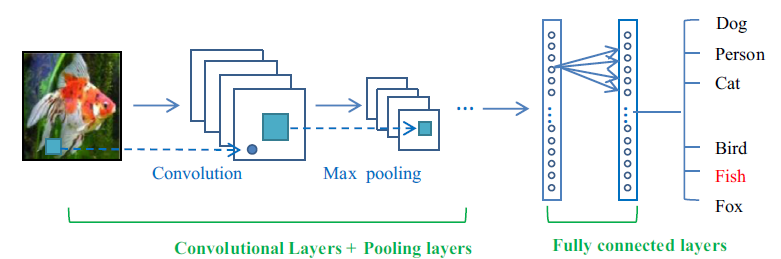
\includegraphics[scale=0.72]{section2/CNNarc.png}
	\caption{
طرح کلی از معماری یک شبکه عصبی کانولوشن
\cite{Guo Y2016}}
\label{CNNarc}
\end{figure}
\newpage
\subsection{ماشین بولتزمن محدود شده}
از لحاظ ساختاری، ماشین بولتزمن محدود شده
\LTRfootnote{Restricted Boltzmann Machines(\lr{RBM})}
یک شبکه عصبی مولد و تصادفی
\LTRfootnote{Generative Stochastic Neural Network}
همراه با محدودیت است. منظور از محدودیت آن است که واحدهای قابل مشاهده
\LTRfootnote{Visible Units}
و واحدهای پنهان
\LTRfootnote{Hidden Units}
یک گراف دو بخشی
\LTRfootnote{Bipartite Graph}،
تشکیل ‌دهند. واضح است که به لایه‌ی شامل واحدهای قابل مشاهده، لایه‌ی قابل مشاهده و به لایه‌ی شامل واحدهای پنهان، لایه پنهان می‌گویند و بر طبق محدویت 
\lr{RBM}
واحدهای یک لایه با هم هیچ‌گونه ارتباطی ندارند. این محدودیت باعث می‌شود الگوریتم‌های آموزش کارآمدتر باشند
\cite{Hinton GE1986}.

\begin{figure}[!h]
\centering
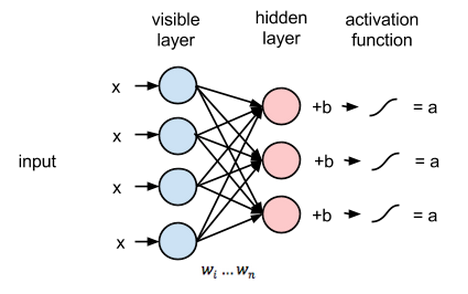
\includegraphics[scale=0.9]{section2/RBM.png}
	\caption{طرح کلی از معماری یک ماشین بولتزمن محدود شده}
\label{RBM}
\end{figure}

مطابق شکل
\ref{RBM}
هدف
\lr{RBM}
بازسازی تا حد امکان دقیق ورودی‌ها است. در مرحله‌ی تغذیه رو به جلو، ورودی‌ها توسط وزن‌ها و اریب‌ها اصلاح و برای فعال‌کردن لایه‌ی پنهان استفاده می‌شوند. از آنجایی که این مدل یک گراف دو بخشی است، واحدهای پنهان
\lr{H} 
و واحدهای قابل مشاهده
\lr{V} 
به‌صورت مشروط مستقل‌اند. بنابراین در معادله زیر:
\begin{equation}
P(HV_1) = P(H_1V_1)P(H_2V_2) ... P(H_nV_1)
\end{equation}
هم
$H$
و هم 
$V_1$
توزیع بولتزمن را برآورده می‌کنند. با ورودی
$V_1$
می‌توانیم
$H $
را از طریق 
$P(HV_1)$
به‌دست آوریم. به‌همین ترتیب می‌توانیم مقدار
$V_2$ 
را از طریق 
$P(HV_2)$
به‌دست آوریم. با تنظیم پارامترها، اختلاف بین
$V_1$
و
$V_2$
را به حداقل می‌رسانیم درنتیجه
$H$
حاصل، به‌عنوان ویژگی خوبی از
$V$
عمل می‌کند. در مقاله 
\cite{Hinton GE1986}
توضیح مبسوطی در این زمینه وجود دارد و راه عملی برای آموزش
\lr{RBM}
توضیح داده شده است.

\subsection{خودرمزنگار}
خودرمزنگار
\LTRfootnote{Autoencoder}
نوع خاصی از شبکه عصبی مصنوعی است که برای رمزگذاری کردن
\LTRfootnote{Encode} 
بهینه یادگیری مورد استفاده قرار می‌گیرد. در ساده‌ترین حالت شامل یک رمزگذار
\LTRfootnote{Encoder}
و یک رمزگشا
\LTRfootnote{Decoder}
به‌همراه فقط یک لایه پنهان می‌باشد. ورودی به رمزگذار داده شده و خروجی از رمزگشا استخراج می‌شود. به‌جای آموزش شبکه و پیش‌بینی مقدار هدف
\lr{Y}
به ازای ورودی
\lr{X}،
یک خودرمزنگار آموزش می‌بینید تا ورودی
\lr{X}
خود را بازسازی کند. بنابراین بردارهای خروجی همان ابعاد بردار ورودی را خواهند داشت.
\begin{figure}[!h]
\centering
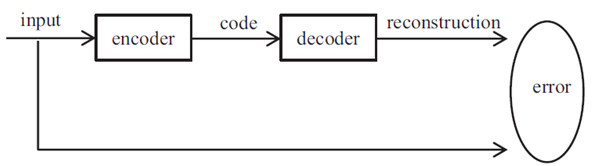
\includegraphics[scale=.8]{section2/autoC.png}
	\caption{فرآیند کلی یک خودرمزنگار\cite{Guo Y2016}}
\label{autoC}
\end{figure}
فرآیند کلی یک خودرمزنگار در شکل
\ref{autoC}
نشان داده شده است. در حین این فرآیند, خودرمزنگار با کمینه‌سازی خطای نوسازی
\LTRfootnote{Reconstruction Error}
بهینه می‌شود. کد متناظر همان ویژگی پیش‌بینی شده است. به‌طورکلی یک لایه‌ی تنها، قادر به دریافت ویژگی‌های متمایز از داده خام نیست. در حال حاضر محققان معمولا از خودرمزنگار عمیق استفاده می‌کنند که کد یادگرفته شده از خودرمزنگار قبلی را به خودرمزنگار بعدی جهت به انجام رساندن کار ارسال می‌کند.


\subsection{کدگذاری تنک}
کدگذاری تنک
\LTRfootnote{Sparse Coding}
نوعی روش بدون سرپرست است که به منظور یادگیری مجموعه خیلی کامل
\LTRfootnote{Over-Complete}
 از توابع پایه برای توصیف داده ورودی مورد استفاده قرار می‌گیرد
\cite{B.A. Olshausen۱997}.
این روش مزیت‌های متعددی دارد به‌عنوان مثال می‌توان به این موارد اشاره کرد :
 
۱) این روش قادر به بازسازی بهتر توصیه‌گر است زیرا از چندین پایه و ارتباط بین توصیه‌گرهای دارای پایه‌های مشترک‌ مشابه، استفاده می‌کند.
  
۲) پراکندگی این اجازه را می‌دهد که خصوصیت‌های برجسته داده ورودی دریافت شوند.

۳) از آنجا که این روش همسو با سیستم بینایی بیولوژیکی است، ویژگی‌های تنک ورودی‌ها نیز برای یادگیری مفید هستند.
   
۴) الگوها با ویژگی‌های تنک از لحاظ خطی بیشتر قابل جداسازی هستند.

برای مقایسه بین این چهار دسته از روش‌های یادگیری عمیق و بدست آوردن درک درستی از آنها، خلاصه‌ای از فواید و مشکلات هریک با توجه به خصوصیات متنوع آنها در جدول 
\ref{methodComp}
آمده است. در این جدول نه خصوصیت کلی وجود دارد. که در آن تعمیم‌پذیری 
\LTRfootnote{Generalization}
اشاره به موثر بودن روش مورد نظر برای سایر ورودی‌ها مانند تصویر, صدا و… و کاربردهای متنوع آنها مثل تشخیص صدا
\LTRfootnote{Speech Recognition}، 
تشخیص تصویر
\LTRfootnote{Visual Recognition} 
و …  دارد.  یادگیری بدون سرپرست 
\LTRfootnote{Unsupervised Learning}
اشاره به توانایی یادگیری خودکار مدل یادگیری عمیق با داده‌های ورودی بدون برچسب و بدون تفسیر نظارتی دارد.  یادگیری ویژگی 
\LTRfootnote{Feature Learning} 
مجموعه‌ای از روش‌هاست که به سیستم امکان اکتشاف خودکار ارائه‌های مورد نیاز برای تشخیص ویژگی یا دسته‌بندی بر اساس داده‌های خام را می‌دهد. زمان واقعی آموزش 
\LTRfootnote{Real-time Training} 
و زمان واقعی پیش‌بینی  
\LTRfootnote{Real-time Prediction}
به‌ترتیب به کارآیی فرآیندهای یادگیری و پیش‌بینی اشاره دارند. ادراک بیولوژیکی 
\LTRfootnote{Biological Understanding}
و توجیه نظری 
\LTRfootnote{Theoretical Justification} 
نشانگر، شالوده بیولوژیکی یا مبانی نظری روش مورد نظر است. تغییرناپذیری 
\LTRfootnote{Invariance}
اشاره به مقاومت روش مورد نظر در مقابل تبدیلاتی مانند دوران، تجانس  و تقارن دارد. مجموعه آموزشی کوچک 
\LTRfootnote{Small Training Set }
اشاره به توانایی یادگیری مدل عمیق با استفاده از تعداد کمی نمونه دارد. این نکته حائز اهمیت است که جدول 
\ref{methodComp} 
فقط یافته‌های کلی کنونی را نمایش می‌دهد و صبحتی از فرصت‌های آینده و یا نمونه‌های اختصاصی نمی‌کند. 


\begin{table}[h!]
\centering
\begin{tabular}{|c|c|c|c|c|}
\hline
خصوصیات       &
\lr{CNN} &  \lr{RBM}  &   \lr{AutoEncoder}  &   \lr{Sparse coding}
\\
\hline

تعمیم‌پذیری&بله & بله & بله & بله
\\
\hline

یادگیری بدون سرپرست&خیر & بله & بله & بله
\\
\hline

یادگیری ویژگی&بله & بله* & بله* & خیر
\\
\hline
 
زمان واقعی آموزش&خیر & خیر & بله & بله
\\
\hline

 زمان واقعی پیش‌بینی&بله & بله & بله & بله
\\
\hline

ادراک بیولوژیکی&خیر & خیر & خیر & بله
\\
\hline

توجیه نظری&بله* & بله & بله & بله
\\
\hline

تغییرناپذیری&بله* & خیر & خیر & بله
\\
\hline

مجموعه آموزشی کوچک&بله* & بله* & بله & بله
\\
\hline
\end{tabular}
	\caption{
مقایسه‌ی روش‌های مختلف شبکه‌های عصبی عمیق
\cite{Guo Y2016}
}
\begin{flushright}
توجه: «بله» اشاره به این دارد که دسته در این خصوصیت به‌خوبی عمل می‌کند. در غیراینصورت با «خیر» علامت‌گذاری می‌شود. «بله*» اشاره به توانایی ابتدایی و یا ضعیف دارد. 
\end{flushright}
	\label{methodComp}
\end{table}

\section{الگوریتم‌های پیشین در مسئله‌ی پیش‌بینی سه‌کلاسه برهم‌کنش دارو - دارو}

در این بخش الگوریتم‌های ارائه شده برای پیش‌بینی سه‌کلاسه برهم‌کنش دارو - دارو معرفی و نحوه‌ی عملکرد آنها به‌صورت مختصر شرح داده ‌می‌شود. هر سه الگوریتم معرفی‌شده، از روش‌های تجزیه ماتریس استفاده می‌کنند. روش تجزیه ماتریس یک مدل توصیه‌گر است که در بخش
\ref{MatFactor}
توضیح داده ‌شده ‌است. این روش با کمی تغییر یک راه‌حل مناسب برای مسئله‌ی پیش‌بینی برهم‌کنش دارو-دارو است که مثال‌هایی از آن در ادامه‌ی این بخش توضیح داده می‌شود.

 لازم به ذکر است که روش پیشنهادی این تحقیق، یک توصیه‌گر مبتنی بر شبکه عصبی عمیق است و از نظر ساختاری هیچ مشابهتی با روش‌های تجزیه ماتریس ندارد. تنها دلیل ذکر این روش‌ها محدود بودن مقالاتی است که در کار خود از داده‌های سه‌کلاسه  استفاده کرده‌اند (نگارنده تا زمان نگارش، این سه مقاله را یافته‌است). درفصل ۴ روند ارزیابی الگوریتم ارائه شده و نتیجه‌ی حاصل با نتایج این مقالات مقایسه می‌شود.


\subsection{چارچوب یکپارچه مبتنی بر تجزیه ماتریس سه‌کلاسه}

ایده اصلی مدل چارچوب یکپارچه مبتنی بر تجزیه ماتریس سه‌کلاسه
\LTRfootnote{Triple Matrix Factorization-Based Unified Framework(\lr{TMFUF})}،
ایجاد ارتباط بین ویژگی‌های داروهای شناخته شده با ساختار گراف برهم‌کنش‌های دارو – دارو است
\cite{Shi J-Y2018}.
چنین ارتباطی را به‌صورت رگرسیون کمترین مربعات جزئی
\LTRfootnote{Partial Least Square Regression}
مدل می‌کند که به‌عنوان یک مدل تجزیه ماتریس سه‌کلاسه
(\lr{TMF})
معرفی شده‌است. برای آموزش مدل رگرسیون از ویژگی عوارض جانبی خارج از برچسب داروها استفاده می‌شود. براساس ادعای نویسندگان این روش اولین روشی است که چارچوب یکپارچه
(\lr{UF})
ارائه می‌دهد. این چارچوب قادر به پیش‌بینی برهم‌کنش‌های دارویی برای هر دو مدل مسئله‌ی دوکلاسه و سه‌کلاسه است.

\begin{figure}[!h]
\centering
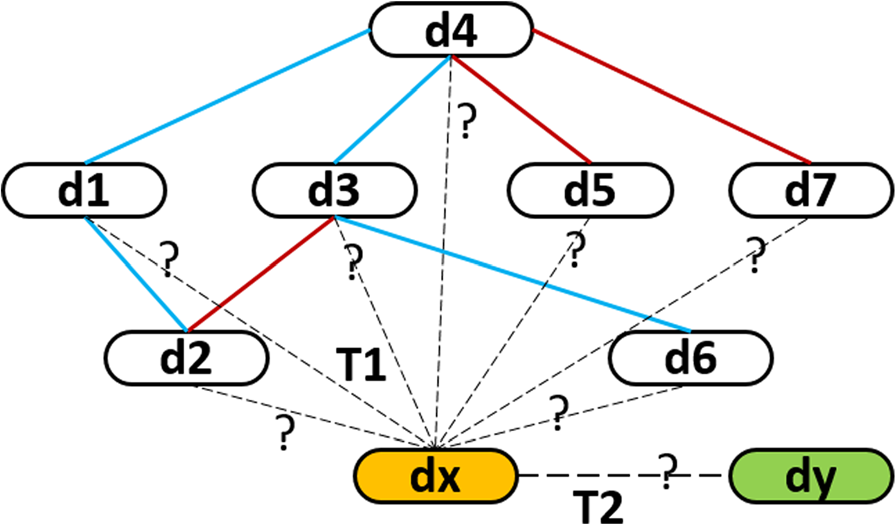
\includegraphics[scale=.5]{section2/TMFUFgraf.png}
	\caption{پیش‌بینی برهم‌کنش \lr{TMFUF}
\cite{Shi J-Y2018}}
\label{TMFUFgraf}
\end{figure}

با توجه به شکل
\ref{TMFUFgraf}
در گراف برهم‌کنش‌، داروها به‌عنوان گره‌ معرفی می‌شوند که داروهای شناخته شده از
$d1$
تا
$d7$
شماره‌گذاری شده‌اند. برهم‌کنش بین داروها با یال‌ها نشان داده می‌شوند و برهم‌کنش افزاینده و کاهنده به‌ترتیب توسط یال‌های قرمز و آبی مشخص شده‌اند. 
$d_x$
و
$d_y$
دو داروی جدید هستند که به‌صورت گره‌های مجزا و به‌ترتیب با برچسب‌های زرد و سبز مشخص می‌شوند. دو نوع پیش‌بینی، که با
$T1$
و
$T2$
برچسب گذاری شده‌اند، با خطوط نقطه‌چین نشان داده می‌شوند.
$T1$
احتمال برهم‌کنش داروی 
$d_x$
با داروهای شناخته‌شده را پیش‌بینی می‌کند، درحالی‌که
$T2$
احتمال برهم‌کنش داروی 
$d_x$
با داروهای جدید
$d_y$
را پیش‌بینی می‌کند. هر دو آنها پیش‌بینی می‌کنند که برهم‌کنش‌های بالقوه باعث افزایش یا کاهش رفتارهای دارویی می‌شوند.

\begin{figure}[!h]
\centering
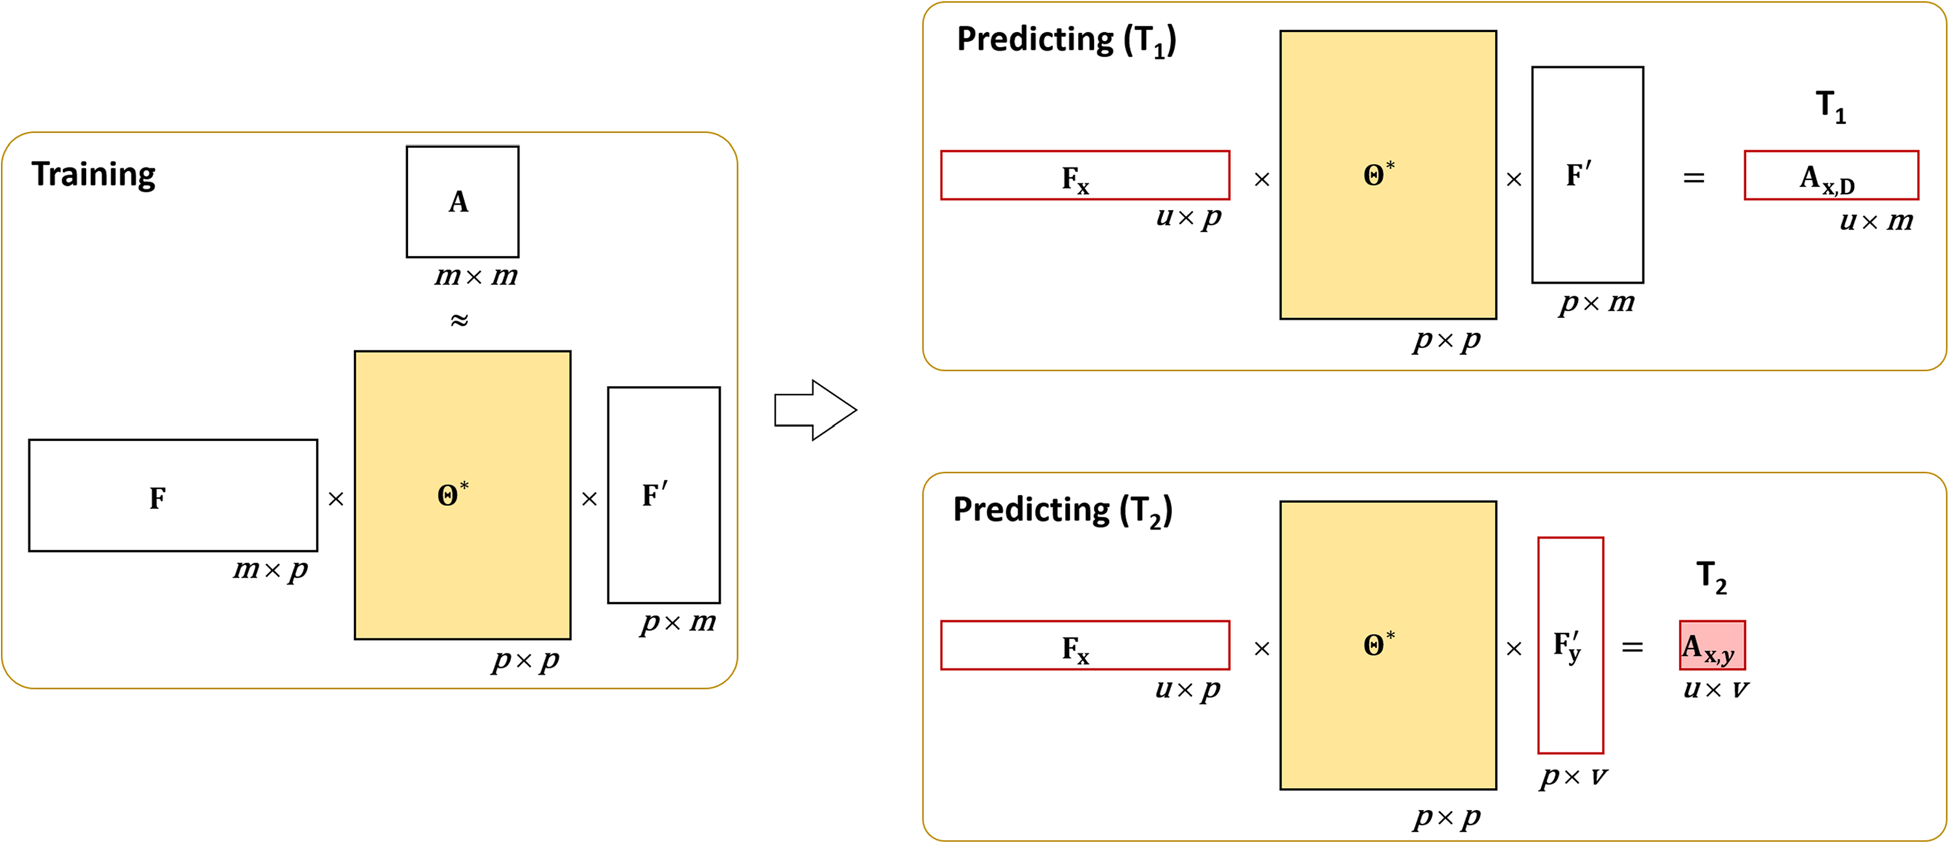
\includegraphics[scale=.3]{section2/TMFUFmodel.png}
	\caption{
ساختار مدل نظارت شده \lr{TMFUF}
\cite{Shi J-Y2018}}
\begin{flushright}
شکل سمت چپ روند آموزش و دو شکل سمت راست دو حالت پیش‌بینی را برای مدل
\lr{TMFUF}
نشان می‌دهند. این مدل برهم‌کنش‌های بین داروهای جدید و داروهای شناخته شده را پیش‌بینی می‌کند (بالا راست). همچنین برهم‌کنش‌های بین داروهای جدید با داروهای جدید را پیش‌بینی می‌کند (پایین راست).
\end{flushright}

\label{TMFUFmodel}
\end{figure}
با توجه به شکل 
\ref{TMFUFmodel}
در مرحله آموزش، ماتریس مجاورت برهم‌کنش‌ها
\lr{A}
و ماتریس ویژگی داروها
\lr{F}،
ماتریس تصویر متقارن
$\Theta$،
با استفاده از یک مدل رگرسیون 
\lr{Bi-Linear}\footnote{رگرسیون دو خطی شیب یک خط رگرسیون برای Y نسبت به X است که به عنوان یک تابع خطی از متغیر سوم Z تغییر می‌کند.}،
به‌صورت زیر ساخته می‌شود.
\begin{equation}
\begin{aligned}
A = F\cdot\Theta\cdot{F^\prime}
\label{TMFUF1}
\end{aligned}
\end{equation}
از آنجا که مقدار 
$\Theta$
را نمی‌توان مستقیما با معکوس‌گیری معادله
\ref{TMFUF1}
به‌دست آورد، بنابراین روش جدیدی برای حل آن پیشنهاد شد. در روش پیشنهادی فرض می‌شود فضای ویژگی نهان کم بعدی وجود دارد که در آن هر دارو توسط یک بردار نهان نشان داده می‌شود و ماتریس حاصل ضرب داخلی بین داروها با ماتریس برهم‌کنش داروها ارتباط مستقیم دارد. به‌علاوه فرض می‌شود ویژگی‌های نهفته داروها با ویژگی مشاهده شده آنها مرتبط است. حل
$\Theta$
به شرح زیر است.
\begin{equation}
\begin{aligned}
\begin{split}
A^*_d= arg min{\parallel{A-{A_d\cdot{A^\prime}_d}\parallel}^2}, 
\\
B^* = arg min{\parallel{{A^*_d} - {F \cdot B}\parallel}^2}
\\
\Theta ^* = B^*\cdot ( B^*) ^ \prime
\end{split}
\end{aligned}
\end{equation}
$A_d$
ماتریس برهم‌کنش پنهان است که هر سطر آن نشان‌دهنده‌ی بردار ویژگی یک دارو در فضای نهفته‌است و باتوجه به متقارن بودن 
\lr{A}، $A_d$
را با الگوریتم تجزیه به مقدار ویژه به‌دست می‌آوریم. 
$A^*_d$
فضای پنهان را با تجزیه ماتریس بازتاب می‌دهد. 
\lr{B}
ماتریس ضرایب رگرسیون است که رابطه‌ای بین فضای ویژگی‌های مشاهده شده و فضای ویژگی پنهان داروها ایجاد می‌کند. برای به‌دست آوردن آن از رگرسیون کم‌ترین مربعات جزئی استفاده می‌شود. 

بعد از
$\Theta^*$،
مدل پیش‌بینی
$T1$
و
$T2$
به شرح زیر استخراج می‌شود.
\begin{equation}
\begin{aligned}
\begin{split}
A_{x,D}={F_x \cdot {\Theta^*}\cdot{F^\prime}},
\\
A_{x,y}={F_x \cdot {\Theta^*}\cdot{F^\prime}_y}
\end{split}
\end{aligned}
\end{equation}

در مدل کردن سه‌کلاسه، تغییرات داروشناسی ناشی از برهم‌کنش‌ها ثبت می‌شود که پیش‌بینی این مدل با ارزش‌تر و از نظر داروشناسی معتبرتر است. علاوه‌براین، راه حلی یکپارچه برای پیش‌بینی برهم‌کنش دارویی در دو سناریو ارائه می‌دهد. در سناریوی اول توانایی مدل برای بازگردانی برهم‌کنش بین داروهای شناخته‌شده سنجیده می‌شود. در سناریوی دوم توانایی مدل برای بازگردانی برهم‌کنش بین داروهای شناخته‌شده و داروی جدید محک می‌خورد. بدیهی است که داروهای جدید با داروهای قبلی هیچ برهم‌کنشی ندارند و اصطلاحا اطلاعات کمتری از آن‌ها وجود دارد. این مدل در هر دو سناریوی مسئله‌ی سه‌کلاسه موظف است نوع برهم‌کنش را پیش‌بینی کند. برهم‌کنش‌های احتمالی جفت داروها افزاینده یا کاهنده هستند. مزیت دیگر روش 
\lr{TMFUF}
در توانایی نشان‌دادن وجود تاثیر معنادار جفت ویژگی‌های دارویی (عوارض جانبی خارج از برچسب هر دو دارو) در پیش‌بینی برهم‌کنش دارویی است.

\subsection{
پیش بینی برهم‌کنش دارو-دارو بر اساس تجزیه ماتریس غیرمنفی}

در روش پیش بینی برهم‌کنش دارو-دارو بر اساس تجزیه ماتریس غیرمنفی
\LTRfootnote{Drug-Drug Interactions Via Semi- None Negative Matrix Factorization} (\lr{DDINMF})
یک مدل نظارت شده برای انجام پیش‌بینی برهم‌کنش دارو-دارو ایجاد می‌شود.
\cite{Yu H2018}

\begin{figure}[!h]
\centering
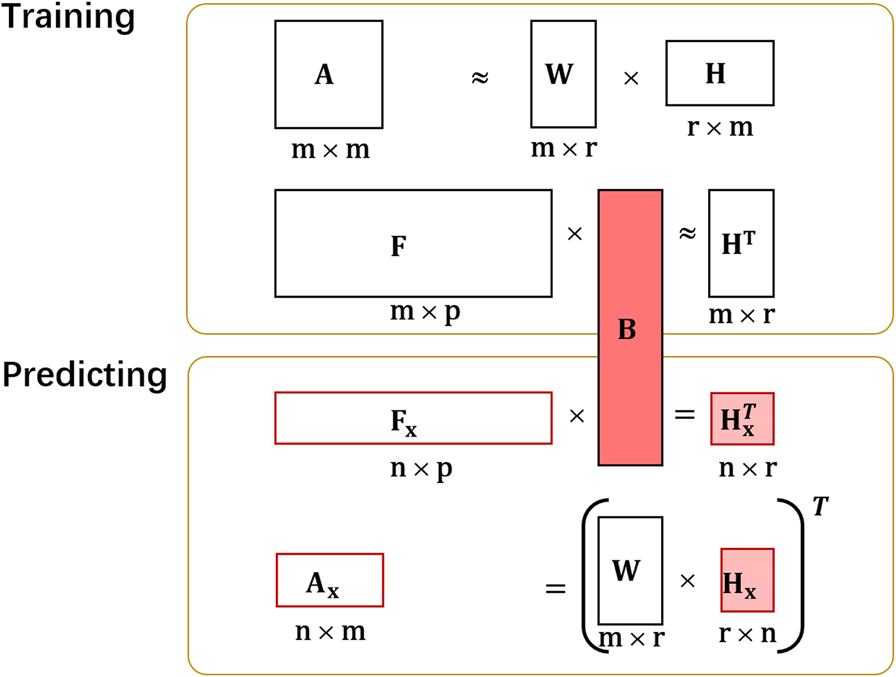
\includegraphics[scale=.4]{section2/DDINMF.png}
	\caption{بررسی اجمالی \lr{DDINMF}
\cite{Yu H2018}}
\label{DDINMF}
\end{figure}
در این روش برهم‌کنش‌ها براساس خواص ساختار شبکه‌ی دارویی  و در روند تجزیه ماتریس آموزش داده می‌شوند. سپس برای ایجاد رابطه بین ویژگی‌های دارویی ( ساختار شیمیایی و عوارض جانبی ) و گراف برهم‌کنش داروها از رگرسیون کم‌ترین مربعات جزئی استفاده می‌شود. این ارتباط در فرآیند پیش‌بینی برهم‌کنش بین داروی جدید و داروهای موجود به‌کار می‌رود. با توجه به شکل
\ref{DDINMF}
مدل 
\lr{DDINMF}
شامل دو مرحله است.

۱) مرحله‌ی آموزش: در این مرحله ماتریس مجاورت ساخته ‌شده بین داروهای شناخته شده به دو ماتریس پایه
\lr{W}
و ماتریس ویژگی پنهان
\lr{H}
توسط 
$A_{m\times m}\approx{W_{m\times r}\times{H_{r\times m}}}$
تجزیه می‌شود. در اینجا 
\lr{r}
اندازه‌ی بعد فضای پنهان است. سپس رابطه‌ای بین ماتریس ویژگی‌ ورودی
\lr{F}
و ماتریس ویژگی پنهان
\lr{H}
توسط رگرسیون به‌صورت 
$(H^T)_{m\times r}={F_{m\times P}\times{B_{p\times r}}}$
مدل می‌شود که 
\lr{B}
ماتریس ضرایب رگرسیون است.

۲) مرحله‌ی پیش‌بینی: در این مرحله، ماتریس ضرایب
\lr{B}
ماتریس ویژگی ورودی داروهای جدید
$F_x$ 
را به ماتریس ویژگی پنهان جدید به‌صورت
${H^T_x}={F_x\times B}$
می‌نگارد
\LTRfootnote{Map}.
سپس با استفاده از ماتریس ویژگی پنهان جدید، پیش‌بینی بین داروهای جدید و داروهای شناخته شده توسط
${A_x}={(W\times{H_x})}^T$
ایجاد می‌شود.

 رویکرد ارائه ‌شده شامل دو روش تجزیه ماتریس غیر منفی
\LTRfootnote{None Negative Matrix Factorization}(\lr{NMF})
 و تجزیه ماتریس نیمه-غیر منفی
\LTRfootnote{Semi- None Negative Matrix Factorization}(\lr{Semi-NMF})
 است. 
 
مدل 
\lr{NMF}
از قید غیرمنفی بودن هر دو ماتریس حاصل از تجزیه استفاده می‌کند تا ماتریس اصلی را تقریب بزند. تابع هدف و تابع‌ بروز‌رسانی
\lr{H} و \lr{W}
به شرح زیر است.
\begin{equation}
\begin{aligned}
min||X-WH||_F^2 =\sum_{i,j}{( x_{ij} -\sum_{k=1}^r w_{ik} h_{ki}})^2, 
W,H\geq0
\end{aligned}
\end{equation}

\begin{equation}
\begin{aligned}
\begin{split}
{w_{ik}}\longleftarrow{w_{ik}\dfrac{(XH^T)_{ik}}{(WHH^T)_{ik}}} 
\\
{h_{ik}}\longleftarrow{h_{ik}\dfrac{(X^TW)_{kj}}{(H^TW^TW)_{kj}}}
\end{split}
\end{aligned}
\end{equation}
که در آن
$w_{ik}$
مراکز خوشه در شبکه‌ی دارویی و
$h_{ik}$
شاخص
\LTRfootnote{Indicator}
خوشه یا عضویت نمونه‌ها در شبکه را مشخص می‌کند.
 
مدل 
\lr{NMF}
محدویت قوی نامنفی بودن را دارد، لذا نمی‌تواند برای حل مسئله‌ی سه‌کلاسه به‌صورت مستقیم استفاده شود. پس لازم است هربار جداگانه روی پیش‌بینی برهم‌کنش‌های افزاینده و کاهنده کار کند. اما مدل
\lr{Semi-NMF}
با استفاده از قید غیرمنفی بودن تنها یکی از ماتریس‌های فضای نهان این امکان را دارد که برای آموزش و پیش‌بینی مسئله‌ی سه‌کلاسه به‌کار رود. روش 
\lr{Semi-NMF}
داروها را خوشه‌بندی کرده و اطلاعات و ویژگی‌های بیشتری از داروها را، درکنار پیش‌بینی برهم‌کنش دارویی، ارائه می‌دهد. در این روش نویسندگان برای پیش‌بینی برهم‌کنش داروهای جدید، از الگوریتم متفاوتی برای به حداقل رساندن تابع هدف استفاده می‌کنند.
\begin{equation}
\begin{aligned}
\begin{split}
{W}\longleftarrow{XH^\dagger}
\\
{H}\longleftarrow{H\odot{\sqrt{\dfrac{(W^TX)^{pos}+[(W^TW)^{neg}H]_{ik}}{(W^TX)^{neg}+[(W^TW)^{pos}H]_{ik}}}}}
\end{split}
\end{aligned}
\end{equation}
که در آن
$H^\dagger$
ماتریس شبه وارون
\lr{H}
است.
$A^{pos}$
و
$A^{neg}$
به ترتیب ماتریس‌هایی هستند که مولفه‌های منفی و مثبت ماتریس 
\lr{A}
را با صفر جایگزین کرده اند:
\begin{equation}
\begin{aligned}
\forall i,j
A_{ij}^{pos}=\dfrac{|A_{ij}|+A_{ij}}{2}  ,   
A_{ij}^{neg}=\dfrac{|A_{ij}|-A_{ij}}{2} 
\end{aligned}
\end{equation}
این رویکرد قادر به پیش‌بینی برهم‌کنش‌های دوکلاسه معمولی و برهم‌کنش‌های جامع سه‌کلاسه است.

از همه مهم‌تر، باید این نکته‌ی کلیدی را درنظر داشته باشیم که شبکه‌ی دوکلاسه برهم‌کنش‌های دارو-دارو به هیچ‌وجه حاوی اطلاعاتی در مورد برهم‌کنش‌های افزاینده و کاهنده نیست، اما بررسی درجه‌ی رئوس در شبکه‌ی سه‌کلاسه جامع اطلاعات مفیدی از انواع برهم‌کنش‌ها ارائه می‌دهد که می‌تواند به درک بهتر برهم‌کنش‌های دارویی بیانجامد. نحوه‌ی چینش برهم‌کنش‌ها در شبکه سه‌کلاسه جامع نشان می‌دهد بروز علائم ناشی از برهم‌کنش‌های افزاینده و کاهنده تصادفی نیست و از قواعد و قوانین خاصی پیروی می‌کند.


گراف سه‌کلاسه‌ی جامع برهم‌کنش یک شبکه با ساختاری متعادل
\LTRfootnote{Structural Balance}
است. نظریه‌ی تعادل ضعیف
\LTRfootnote{Weakly Balance Theorem}
بیان می‌کند که گره‌های شبکه‌ را می‌توان در
\lr{k}
خوشه قرار داد، به‌طوری که اکثر یال‌های درون هر خوشه افزاینده و اکثر یال‌های بین خوشه‌ها کاهنده باشند
\cite{Davis1967}.


\subsection{تنظیم متعادل تجزیه ماتریس نیمه غیر منفی}

روش موسوم به تنظیم متعادل تجزیه ماتریس نیمه غیر منفی
\cite{Shi J2019} 
\LTRfootnote{Balance Regularized Semi-Nonnegative Matrix Factorization} (\lr{BRSNMF})
تلاشی برای تقویت روش
\lr{Semi-NMF}
پیشین است و علاوه بر آن ساختار اساسی تعادل ضعیف شبکه جامع سه‌کلاسه را نشان می‌دهد. این مدل از روابط ساختاری برای حل دو مسئله استفاده می‌کند: 
 
۱) کشف انجمن\LTRfootnote{Community}‌های دارویی و تقویت توان انجمن‌یابی
\LTRfootnote{Community Detection}

۲) پیش‌بینی جامع برهم‌کنش‌ها. 

طبق پیش‌بینی نویسندگان مقاله، شبکه‌ی برهم‌کنش دارویی را می‌توان به انجمن‌ها و گروه‌هایی تقسیم‌بندی کرد. به‌شکلی بیشتر یال (برهم‌کنش) های درون انجمن دارویی افزاینده و بیشتر یال‌های بین انجمنی کاهنده باشند. در این راستا دو معیار تنظیم گراف،
$Gr_1$
برای درون انجمن‌ها و
$Gr_2$
برای بین انجمن‌ها به‌صورت زیر معرفی شدند . همچنین، این دو معیار تنظیم از به وجود آمدن خوشه‌هایی با گره‌های کم جلوگیری می‌کنند.
\begin{equation}
\begin{aligned}
\begin{split}
Gr_1 = min \sum^k_{c=1}\dfrac{{h^T_c}{A^-}{h_c}}{{h^T_c}{h_c}},
\\
Gr_2 = min \sum^k_{c=1}\dfrac{{h^T_c}{L^+}{h_c}}{{h^T_c}{h_c}}
\end{split}
\end{aligned}
\end{equation}
که درآن
$h_c$,\lr{c}امین
ستون برداری در 
\lr{H}
است و 
$L^+=D^+-A^+$
است که در آن
$D^+$
ماتریس قطری
$A^+$
است و داریم
$\forall i,j a^+_{ij}=\dfrac{|a_{ij}|+a_{ij}}{2} , a^-_{ij}=\dfrac{|a_{ij}|-a_{ij}}{2}$.

با ترکیب 
$Gr_1$
و
$Gr_2$
و پس از ساده‌سازی داریم:
\begin{equation}
\begin{aligned}
Gr \equiv max { tr(H^T(\sigma I-\eta (A^-+L^+))H)}=max{ tr(G)}
\end{aligned}
\end{equation}
که در آن
$\sigma,\eta>0$
اندازه خوشه‌ها را کنترل می‌کند.

همچنین، معیار تنظیم 
\lr{Sr}
برای کنترل پراکندگی
\lr{H}
به‌صورت زیر طوری تعریف می‌شود که گره‌های دارو در شبکه برهم‌کنش به کمترین انجمن‌های ممکن تعلق داشته باشند:
\begin{equation}
\begin{aligned}
Sr= \sum^m_j||h_j||_1^2 =tr(HlH^T)=tr(s)
\end{aligned}
\end{equation}
که در آن
\lr{l}
ماتریس
$k \times k$
یی است که تمام درآیه‌های آن یک است.

پس از یکپارچه‌سازی معیارهای تنظیم به ماتریس درجه پایین، تابع هدف 
\lr{BRSNMF}
به شرح زیر است.
\begin{equation}
\begin{aligned}
min||A-WH^T||_F^2 +\alpha \cdot tr(S) - \beta \cdot tr(G), 
h_{ij}\geq0 , \forall i,j \in [1,...,m]
\end{aligned}
\end{equation}
برای حل و بروز‌رسانی از قوانین زیر استفاده می‌شود.
\begin{equation}
\begin{aligned}
\begin{split}
{W}\longleftarrow{AH(H^TH)^{-1}}
\\
{H}\longleftarrow{H\odot(N\div D)^{\dfrac{1}{2}}}
\\
N=(A^TW)_++(HW^TW)_-+\beta \eta(L^+H)_-+\beta \sigma H
\\
D=(A^TW)_-+(HW^TW)_+\alpha Hl+\beta \eta A^-H+\beta\eta(L^+H)_+
\end{split}
\end{aligned}
\end{equation}
که عملگرهای
$X_+$
و
$X_-$
بصورت
$X_+=\dfrac{|A|+A}{2}$
و
$X_-=\dfrac{|A|-A}{2}$
تعریف می‌شوند.


این تغییرات دو خصوصیت زیر را به نتایج حاصل از اجرای روش تحمیل کرد. 
 
۱) ارتباطات بین انجمنی بیشتر از نوع کاهنده باشد که کمک کند دورهای متعادل در درون انجمن‌ها تشکیل شده و دورهای نامتعادل در بین انجمن‌ها باشد. 

۲) از ایجاد خوشه‌هایی با تعداد گره‌های کم جلوگیری شود که باعث شد نسبت به
\lr{Semi-NMF}
انجمن‌های خیلی چاق یا خیلی لاغر تشکیل نشود. 

\begin{figure}[!h]
\centering
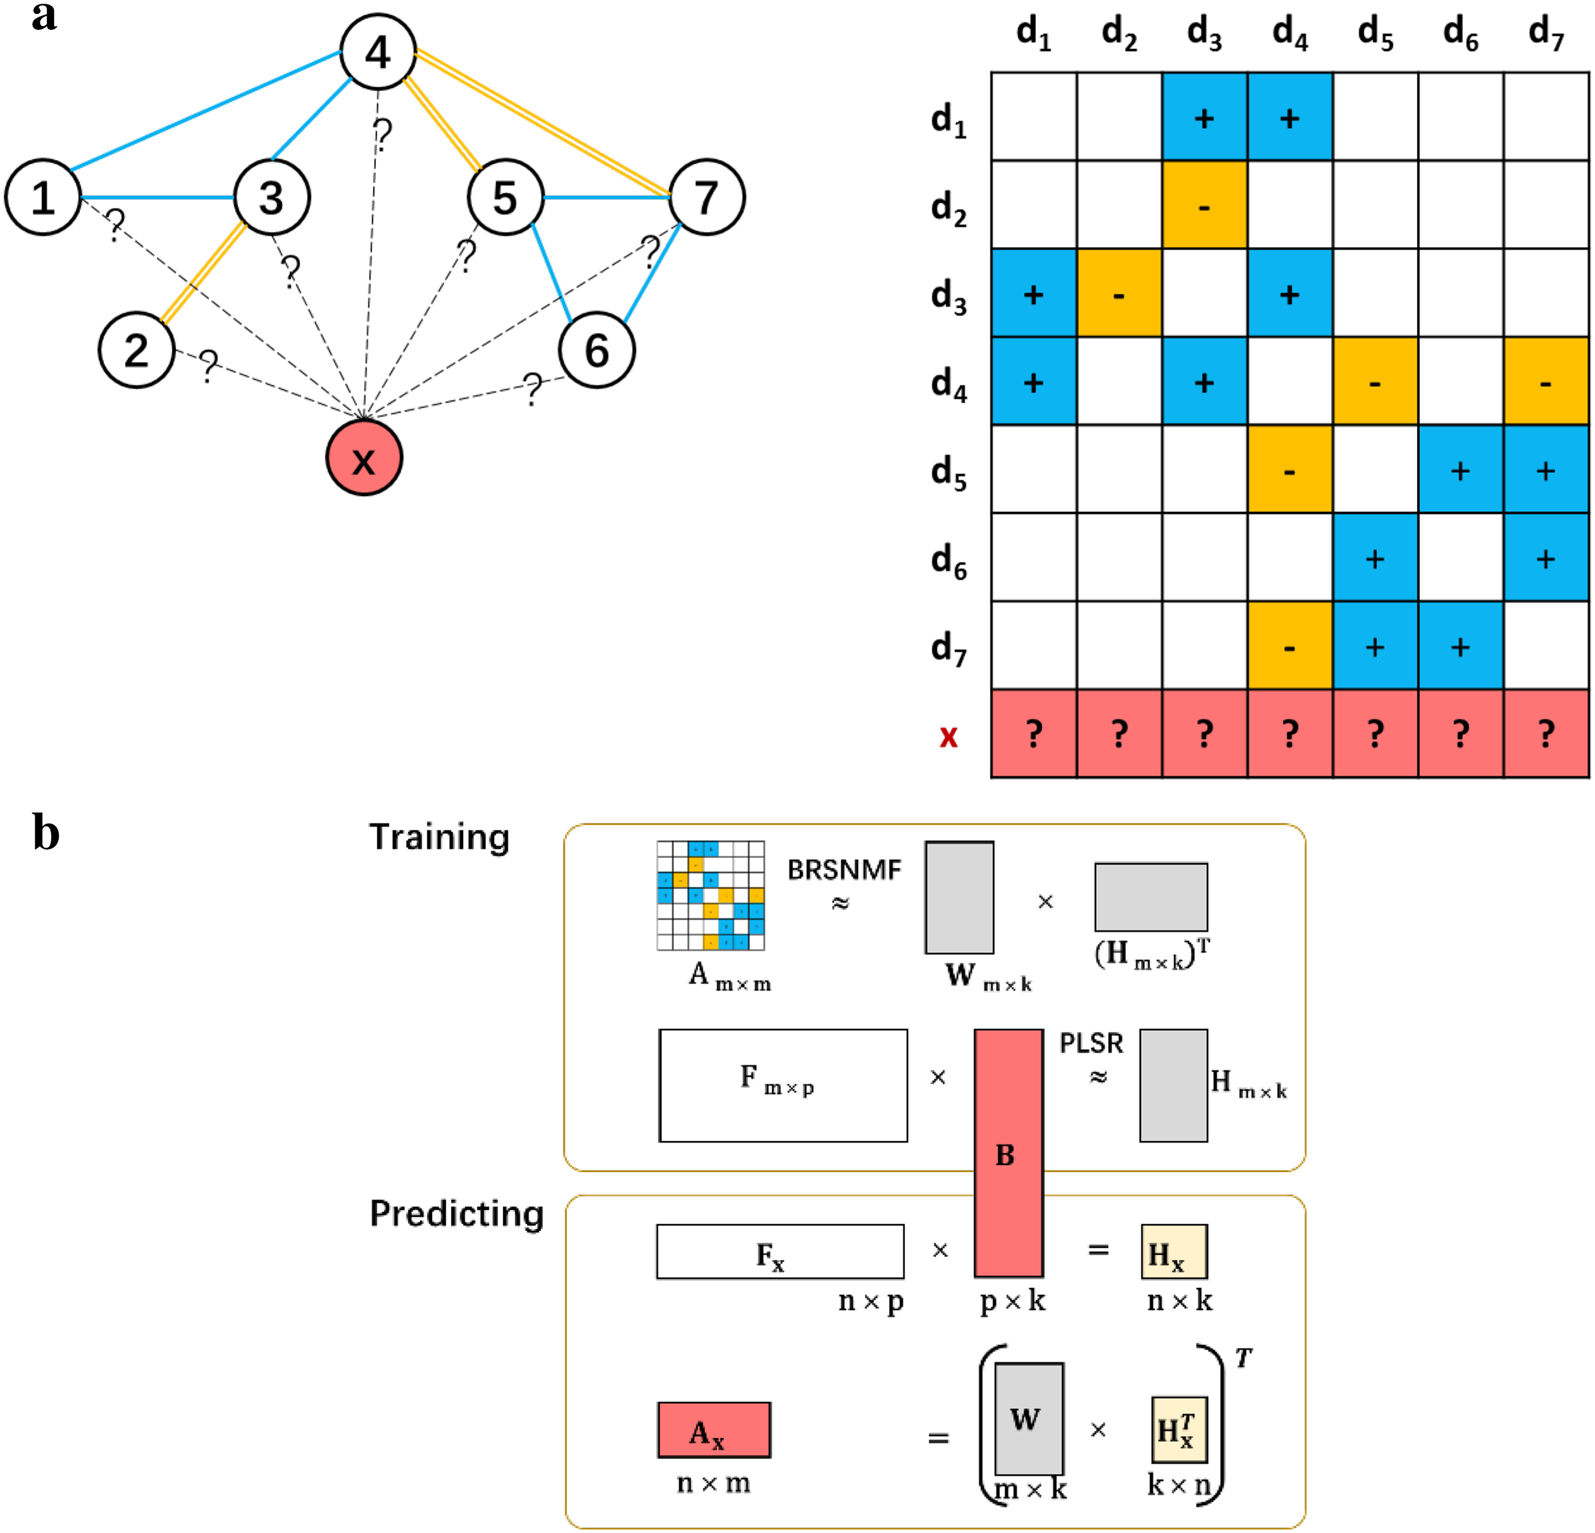
\includegraphics[scale=.3]{section2/BRSNMF.png}
	\caption{پیش‌بینی برهم‌کنش جامع در سناریو شروع سرد \lr{BRSNMF}
\cite{Shi J2019}}
\label{BRSNMF}
\end{figure}

اتخاذ چارچوب مسئله شروع سرد
\LTRfootnote{Cold Start}\cite{Yu H2018}
در رویکرد مبتنی بر
\lr{BRSNMF}
در سناریو پیش‌بینی برهم‌کنش برای داروی جدید، شامل دو مرحله به شرح زیر است که در شکل
\lr{b}\ref{BRSNMF}
نشان داده شده است.

1) در مرحله آموزش، رویکرد تجزیه ماتریس 
$A_{m \times m} \approx W_{m \times k}\times (H_{m\times k})^T$
توسط
\lr{BRSNMF}
و رگرسیون خطی 
$H_{m\times k}=F_{m \times p}\times B_{p \times k}$
توسط رگرسیون کمترین مربعات جزئی به‌دست آمد.

2) در مرحله پیش‌بینی، ماتریس ضرایب آموزش داده شده
$B_{p \times K}$
در ابتدا ماتریس ویژگی
$F_x$ 
را به فضای پنهان
$n\times k$
به‌صورت
${H_x}={F_x\times B}$
می‌نگارد. سپس برهم‌کنش پیش‌بینی شده
$n\times m$
بین داروهای جدید و داروهای تایید شده توسط 
${A_x} = {H_xW^T} = {(F_xB)W^T}$
محاسبه می‌شود. در این مرحله از ویژگی پروتئین‌های مرتبط به دارو
\LTRfootnote{Drug Binding Protein(\lr{DBP})}
استفاده می‌کند.

 نتایج نشان می‌دهند که
\lr{BRSNMF}
انجمن‌های دارویی ایجاد می‌کند که دارای اندازه‌های مناسب‌تری هستند، خاصیت تعادلی ضعیف بیشتر و اهمیت دارویی دارند. 


در این فصل سعی شد پیش‌نیازهای محاسباتی و الگوریتم‌های سامانه‌های توصیه‌گر و یادگیری عمیق معرفی شوند. همچنین الگوریتم‌های مرتبط که قبلا روی این مسئله کار کرده بودند معرفی و بررسی شدند. در ادامه و در فصل بعد روند آماده‌سازی داده برای ورودی دادن به روش و همچنین پیاده‌سازی روش بیان می‌شود.

